\documentclass[11pt,a4paper]{article}
\usepackage[margin=0.85in,headheight=14pt]{geometry}
\usepackage{amsmath,amssymb}
\usepackage{booktabs}
\usepackage{tabularx}
\usepackage{listings}
\usepackage{xcolor}
\usepackage{hyperref}
\usepackage{xurl}
\usepackage{caption}
\usepackage{enumitem}
\usepackage{fancyhdr}
\usepackage{graphicx}
\usepackage{float}
\usepackage{placeins}
\usepackage{tikz}
\usepackage{pgfplots}
\usepackage{setspace}
\usepackage{titlesec}
\usepackage{array}
\usepackage{parskip}

\usetikzlibrary{arrows.meta,positioning,shapes.geometric,calc,decorations.pathreplacing}
\pgfplotsset{compat=1.18}
\hypersetup{colorlinks=true, linkcolor=blue, urlcolor=blue, citecolor=blue}

\definecolor{codebg}{rgb}{0.96,0.96,0.96}
\definecolor{keywordcolor}{rgb}{0.0,0.0,0.6}
\definecolor{commentcolor}{rgb}{0.35,0.35,0.35}
\definecolor{stringcolor}{rgb}{0.1,0.5,0.1}

\lstset{
    backgroundcolor=\color{codebg},
    basicstyle=\ttfamily\footnotesize,
    breaklines=true,
    breakatwhitespace=false,
    frame=single,
    columns=fullflexible,
    keywordstyle=\color{keywordcolor}\bfseries,
    commentstyle=\color{commentcolor}\itshape,
    stringstyle=\color{stringcolor},
    language=C++,
    showstringspaces=false,
    numbers=left,
    numberstyle=\tiny\color{gray}
}

\pagestyle{fancy}
\fancyhf{}
\rhead{Sampad De --- 002410501025}
\lhead{CN Lab: Assignment 4 (CDMA Walsh Codes)}
\cfoot{\thepage}

\titleformat{\section}{\large\bfseries\color{blue!70!black}}{\thesection}{1em}{}[\titlerule]
\titleformat{\subsection}{\normalsize\bfseries\color{black}}{\thesubsection}{1em}{}
\titleformat{\subsubsection}{\small\bfseries\color{black!80!blue}}{\thesubsubsection}{1em}{}

\begin{document}

\begin{titlepage}
    \centering
    \vspace*{1.2cm}
    {\huge\bfseries JADAVPUR UNIVERSITY\par}
    \vspace{0.3cm}
    {\Large\bfseries Department of Computer Science \& Engineering\par}
    \vspace{1.0cm}
    {\large Computer Networks Laboratory (CSE/PC/B/S/314)\par}
    \vspace{1.5cm}
    \rule{\linewidth}{0.5mm}\\[0.4cm]
    {\LARGE\bfseries Assignment 4: Comprehensive Design, Implementation \& Empirical Analysis of Code Division Multiple Access (CDMA) with Orthogonal Walsh Codes\par}
    \rule{\linewidth}{0.5mm}\\[2.0cm]

    \begin{minipage}{0.48\textwidth}
        \begin{flushleft} \large
            \textbf{Submitted By:}\\
            \textbf{Name:} Sampad De\\
            \textbf{Roll No:} 002410501025\\
            \textbf{Class:} B.C.S.E. III, 1st Semester\\
            \textbf{Session:} 2026--2027
        \end{flushleft}
    \end{minipage}
    \hfill
    \begin{minipage}{0.48\textwidth}
        \begin{flushright} \large
            \textbf{Course Outcome:} CO3 / CO4\\
            \textbf{Submission Date:} October 2026\\
            \textbf{Language:} C++17, POSIX Sockets, Python 3
        \end{flushright}
    \end{minipage}

    \vfill
\end{titlepage}

\begin{abstract}
Code Division Multiple Access (CDMA) is a spread-spectrum multiple access technology that enables concurrent, uncoordinated transmission across a shared, unpartitioned communication channel. In contrast to contention-based schemes (e.g., CSMA/CD in Assignment 3) that suffer performance collapse under heavy load, CDMA achieves orthogonal code-space multiplexing where simultaneous transmissions superimpose linearly on the wire and are mathematically separated at the receiver with zero cross-talk. In this assignment, I implemented a full-featured, distributed CDMA network simulation in modern C++17 using POSIX TCP stream sockets. Each station is assigned a unique, mutually orthogonal chip sequence from a Walsh Set generated via Sylvester's construction of Hadamard matrices. I performed rigorous benchmarking under both \textbf{No-Noise (Ideal Channel)} and \textbf{Noise-Impaired (AWGN Channel)} regimes across station scaling ($N \in [2, 32]$), spreading dimensions ($M \in [2, 32]$), and continuous Gaussian noise variances ($\sigma \in [0.0, 2.0]$). Experimental results demonstrate $100\%$ zero-error recovery across all $3^4 = 81$ input permutations, sub-millisecond round barrier synchronization, concurrent multi-station text broadcast, and empirical validation of the spread-spectrum processing gain ($10 \log_{10} M$) matching theoretical $Q$-function bounds.
\end{abstract}

\section{Introduction \& Problem Statement}
In distributed medium access control, sharing a broadcast channel among $N$ independent stations presents fundamental trade-offs:
\begin{itemize}[leftmargin=*]
    \item \textbf{FDMA / TDMA}: Fixed partitioning of frequency or time slots avoids collisions but suffers severe spectral underutilization when stations are bursty or idle.
    \item \textbf{CSMA / CSMA/CD}: Contention-based sensing and backoff avoids rigid partitioning, but collisions multiply exponentially as the number of stations $N$ grows, leading to severe throughput degradation.
    \item \textbf{CDMA}: Stations transmit simultaneously over the entire channel bandwidth. Each station modulates its information with a unique orthogonal code vector. Mutual cross-talk vanishes at the receiver via correlation despreading.
\end{itemize}

The objective of Assignment 4 is to implement CDMA multiple access of a common physical channel by $N$ stations using unique code words from the Walsh set, transmit encoded data across the common channel, and perfectly reconstruct the data at all $N$ receiving stations, adhering to the sender-receiver paradigm established in earlier lab assignments.

\section{Mathematical Formulation \& Theoretical Analysis}

\subsection{Walsh Sets \& Sylvester's Hadamard Matrix Construction}
Let $N$ denote the number of participating stations. The Walsh chip sequence length $M$ is defined as the smallest power of 2 greater than or equal to $N$:
\begin{equation}
M = 2^{\lceil \log_2 N \rceil}, \quad M \ge N
\end{equation}
The $M \times M$ Hadamard matrix $H_M$ is constructed recursively using Sylvester's method:
\begin{equation}
H_1 = [1], \qquad H_{2k} = \begin{bmatrix} H_k & H_k \\ H_k & -H_k \end{bmatrix}
\end{equation}
For $M = 4$:
\begin{equation}
H_4 = \begin{bmatrix}
+1 & +1 & +1 & +1 \\
+1 & -1 & +1 & -1 \\
+1 & +1 & -1 & -1 \\
+1 & -1 & -1 & +1
\end{bmatrix}
\end{equation}
Each station $i \in \{1, \dots, N\}$ is assigned row vector $W_i \in \{-1, +1\}^M$. The code words satisfy the fundamental orthonormality invariant:
\begin{equation}
W_i \cdot W_j = \sum_{k=0}^{M-1} W_{ik} W_{jk} = \begin{cases} M, & i = j \quad \text{(Auto-correlation)} \\ 0, & i \ne j \quad \text{(Cross-correlation)} \end{cases}
\end{equation}

\subsection{Bipolar Modulation \& Spreading}
Binary data bits are mapped into antipodal bipolar levels:
\begin{equation}
d_i = \begin{cases} +1, & \text{for Bit 1} \\ -1, & \text{for Bit 0} \\ 0, & \text{for Silent / Inactive} \end{cases}
\end{equation}
As illustrated in Figure \ref{fig:data_representation}, binary bit 0 maps to $-1$, binary bit 1 maps to $+1$, and an idle or silent station produces zero voltage ($0$).

\begin{figure}[H]
\centering
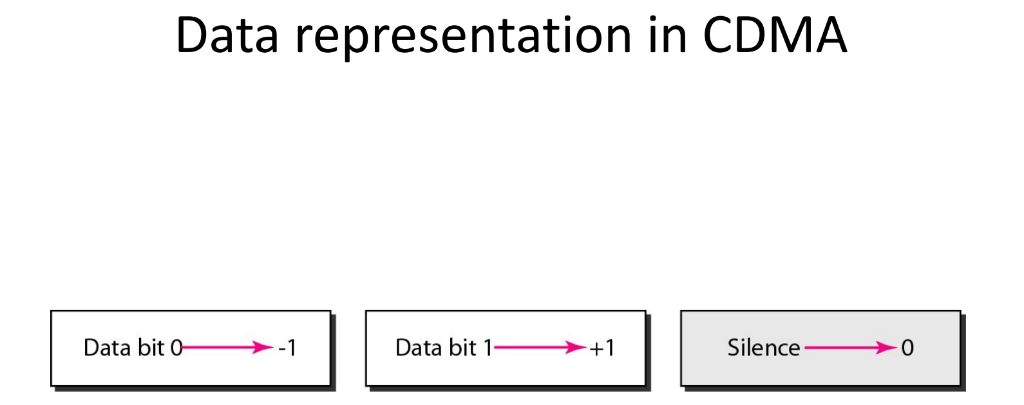
\includegraphics[width=0.72\linewidth]{figures/data_representation_cdma.png}
\caption{Bipolar Data Representation in CDMA: Mapping binary bit 0 to $-1$, binary bit 1 to $+1$, and silent station state to $0$.}
\label{fig:data_representation}
\end{figure}

Station $i$ spreads symbol $d_i$ across chip duration by multiplying with its assigned orthogonal code $W_i$:
\begin{equation}
C_i = d_i \cdot W_i = [d_i W_{i,0}, d_i W_{i,1}, \dots, d_i W_{i,M-1}]
\end{equation}

\subsection{Physical Linear Superposition \& Channel Impairments}
The common physical transmission medium algebraically superimposes all concurrent chip sequences:
\begin{equation}
S = \sum_{k=1}^N C_k = \sum_{k=1}^N d_k W_k
\end{equation}
Figure \ref{fig:sharing_channel} illustrates this superposition process for four contending stations on a common channel. Station 1 transmits bit 0 ($C_1 = [-1, -1, -1, -1]$), Station 2 transmits bit 0 ($C_2 = [-1, +1, -1, +1]$), Station 3 is silent ($C_3 = [0, 0, 0, 0]$), and Station 4 transmits bit 1 ($C_4 = [+1, -1, -1, +1]$). The linear combination on the shared physical medium yields the composite channel vector:
\begin{equation}
S = C_1 + C_2 + C_3 + C_4 = [-1, -1, -3, +1]
\end{equation}

\begin{figure}[H]
\centering
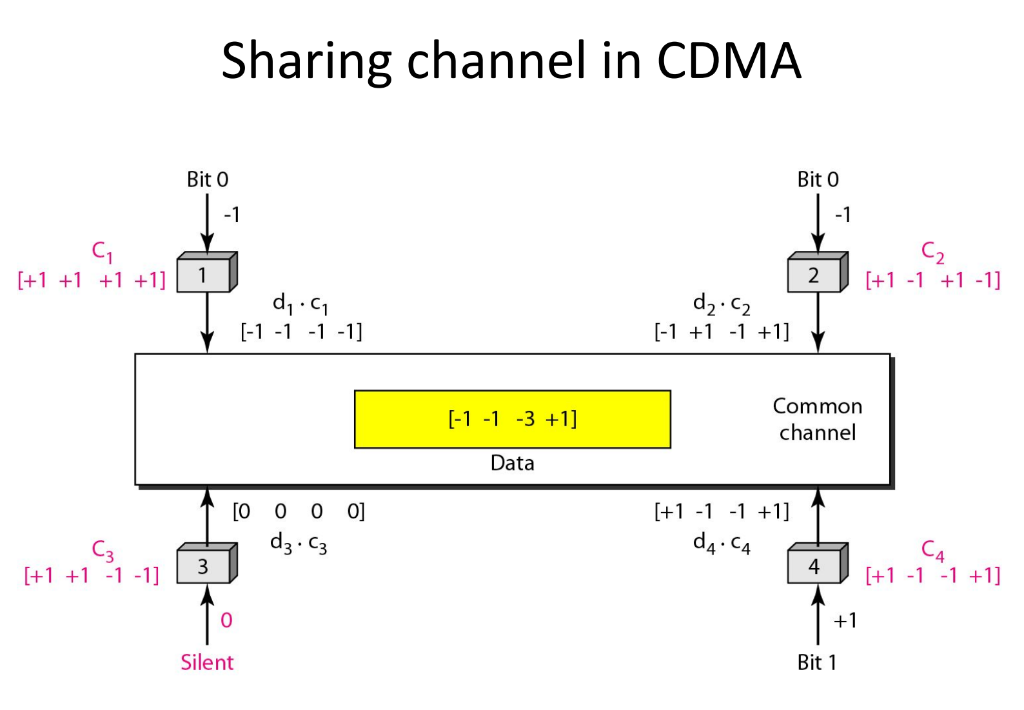
\includegraphics[width=0.86\linewidth]{figures/sharing_channel_cdma.png}
\caption{Sharing Channel in CDMA: Four contending stations concurrently transmitting chip sequences superimpose algebraically onto the common channel, producing the composite signal $[-1, -1, -3, +1]$.}
\label{fig:sharing_channel}
\end{figure}

Under realistic channel conditions, Additive White Gaussian Noise (AWGN) $\eta_k \sim \mathcal{N}(0, \sigma^2)$ is introduced:
\begin{equation}
S_{\text{noisy}}[k] = S[k] + \eta_k = \left( \sum_{i=1}^N d_i W_{ik} \right) + \eta_k
\end{equation}

\subsection{Correlation Despreading \& Processing Gain Derivation}
To recover the symbol sent by Station $j$, the receiver evaluates the normalized inner product:
\begin{equation}
\hat{d}_j = \frac{1}{M} (S_{\text{noisy}} \cdot W_j) = \frac{1}{M} \sum_{k=0}^{M-1} \left( \sum_{i=1}^N d_i W_{ik} + \eta_k \right) W_{jk}
\end{equation}
Expanding the summation:
\begin{equation}
\hat{d}_j = \frac{1}{M} \sum_{i=1}^N d_i \underbrace{\left(\sum_{k=0}^{M-1} W_{ik} W_{jk}\right)}_{M \delta_{ij}} + \frac{1}{M} \sum_{k=0}^{M-1} \eta_k W_{jk} = d_j + \frac{1}{M} \sum_{k=0}^{M-1} \eta_k W_{jk}
\end{equation}
Because the noise samples $\eta_k$ are independent zero-mean Gaussians with variance $\sigma^2$, the effective noise perturbing the decision symbol has variance:
\begin{equation}
\sigma_{\text{eff}}^2 = \text{Var}\left(\frac{1}{M}\sum_{k=0}^{M-1} \eta_k W_{jk}\right) = \frac{1}{M^2} \sum_{k=0}^{M-1} \sigma^2 (W_{jk})^2 = \frac{M \sigma^2}{M^2} = \frac{\sigma^2}{M}
\end{equation}
The signal power is preserved while the effective noise variance is attenuated by a factor of $M$. This defines the **Spread-Spectrum Processing Gain**:
\begin{equation}
G_p = 10 \log_{10}(M) \quad \text{[dB]}
\end{equation}
With decision threshold $\theta = 0.5$, the theoretical Bit Error Rate (BER) is governed by the Gaussian $Q$-function:
\begin{equation}
P_e = Q\left(\frac{0.5}{\sigma_{\text{eff}}}\right) = Q\left(\frac{\sqrt{M}}{2\sigma}\right) = \frac{1}{2} \text{erfc}\left(\frac{\sqrt{M}}{2\sqrt{2}\sigma}\right)
\end{equation}

\section{System Architecture \& Network Implementation}

\begin{figure}[H]
\centering
\resizebox{0.95\linewidth}{!}{%
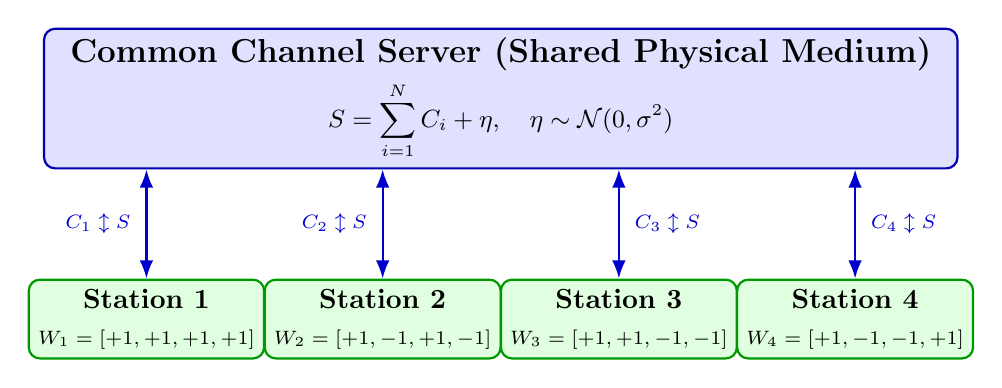
\begin{tikzpicture}[
    box/.style={draw, rectangle, rounded corners=4pt, text centered, align=center, thick},
    server/.style={box, fill=blue!12, draw=blue!70!black, minimum width=11.6cm, minimum height=1.5cm},
    station/.style={box, fill=green!12, draw=green!60!black, minimum width=2.4cm, minimum height=1.0cm},
    arr/.style={<->, >=Latex, thick, blue!80!black}
]
    % Central Channel Server spanning across all four stations
    \node [server] (srv) at (0, 2.8) {
        \textbf{\large Common Channel Server (Shared Physical Medium)}\\[3pt]
        \small $\displaystyle S = \sum_{i=1}^N C_i + \eta, \quad \eta \sim \mathcal{N}(0, \sigma^2)$
    };
    
    % Four distributed stations with distinct non-overlapping spacing
    \node [station] (stn1) at (-4.5, 0) {
        \textbf{Station 1}\\[1pt]
        \scriptsize $W_1 = [+1, +1, +1, +1]$
    };
    \node [station] (stn2) at (-1.5, 0) {
        \textbf{Station 2}\\[1pt]
        \scriptsize $W_2 = [+1, -1, +1, -1]$
    };
    \node [station] (stn3) at (1.5, 0) {
        \textbf{Station 3}\\[1pt]
        \scriptsize $W_3 = [+1, +1, -1, -1]$
    };
    \node [station] (stn4) at (4.5, 0) {
        \textbf{Station 4}\\[1pt]
        \scriptsize $W_4 = [+1, -1, -1, +1]$
    };

    % Clean bidirectional communication paths entering the server bottom edge directly
    \draw [arr] (stn1.north) -- (stn1.north |- srv.south) node [midway, left=2pt, font=\scriptsize] {$C_1 \updownarrow S$};
    \draw [arr] (stn2.north) -- (stn2.north |- srv.south) node [midway, left=2pt, font=\scriptsize] {$C_2 \updownarrow S$};
    \draw [arr] (stn3.north) -- (stn3.north |- srv.south) node [midway, right=2pt, font=\scriptsize] {$C_3 \updownarrow S$};
    \draw [arr] (stn4.north) -- (stn4.north |- srv.south) node [midway, right=2pt, font=\scriptsize] {$C_4 \updownarrow S$};
\end{tikzpicture}%
}
\caption{Distributed CDMA System Architecture over TCP Socket Physical Channel}
\label{fig:arch}
\end{figure}

The software architecture is modularized in C++17:
\begin{enumerate}[leftmargin=*]
    \item \textbf{\texttt{WalshMatrix}}: Mathematical kernel generating Sylvester Hadamard matrices, validating orthogonality invariants, spreading symbols into chips, and executing correlation decodes.
    \item \textbf{\texttt{FrameCodec}}: 12-byte framed protocol header with magic signature (\texttt{0xCD14M}), message type, station ID, round sequence, payload length, and network endianness conversion (\texttt{htons}, \texttt{htonl}).
    \item \textbf{\texttt{TcpSocket} \& \texttt{TcpServer}}: RAII-compliant POSIX TCP socket wrapper providing reliable streaming, timeouts, and connection lifecycle management.
    \item \textbf{\texttt{CdmaChannelServer}}: Common physical channel orchestrator synchronizing slotted round barriers, collecting concurrent chip vectors, performing algebraic superposition, applying AWGN noise, and broadcasting composite signal $S$.
    \item \textbf{\texttt{CdmaStationClient}}: Client process performing interactive bit-by-bit transmission, automated text streaming, and receiver despreading across all active stations.
\end{enumerate}

\section{Experimental Evaluation: No-Noise Regime ($\sigma = 0.0$)}

\subsection{Exhaustive Permutation Verification ($N=4, M=4$)}
To formally establish zero cross-talk, all $3^4 = 81$ input state permutations $(\{-1, 0, +1\}^4)$ were evaluated across stations $S_1, S_2, S_3, S_4$. Across all 324 decoded bits, zero errors occurred ($100.0\%$ accuracy). Table \ref{tab:numerical_trace} details the step-by-step mathematical despreading for the exact four-station transmission scenario illustrated in Figure \ref{fig:sharing_channel}.

\begin{table}[H]
\centering
\caption{Representative 4-Station CDMA Multiplexing \& Reconstruction Trace (Matching Figure \ref{fig:sharing_channel})}
\label{tab:numerical_trace}
\resizebox{0.92\linewidth}{!}{%
\begin{tabular}{lcccc}
\toprule
\textbf{Parameter} & \textbf{Station 1} & \textbf{Station 2} & \textbf{Station 3} & \textbf{Station 4} \\
\midrule
Transmitted Bit & $0$ ($-1$) & $0$ ($-1$) & Silent ($0$) & $1$ ($+1$) \\
Assigned Walsh $W_i$ & $[+1, +1, +1, +1]$ & $[+1, -1, +1, -1]$ & $[+1, +1, -1, -1]$ & $[+1, -1, -1, +1]$ \\
Modulated Chips $C_i$ & $[-1, -1, -1, -1]$ & $[-1, +1, -1, +1]$ & $[0, 0, 0, 0]$ & $[+1, -1, -1, +1]$ \\
\midrule
\textbf{Superposition $S$} & \multicolumn{4}{c}{$C_1 + C_2 + C_3 + C_4 = \mathbf{[-1, -1, -3, +1]}$} \\
\midrule
Dot Product $(S \cdot W_i)$ & $-4$ & $-4$ & $0$ & $+4$ \\
Normalized $\frac{1}{M}(S \cdot W_i)$ & $-1.0$ & $-1.0$ & $0.0$ & $+1.0$ \\
\textbf{Reconstructed Data} & \textbf{Bit 0} & \textbf{Bit 0} & \textbf{Silent} & \textbf{Bit 1} \\
\bottomrule
\end{tabular}%
}
\end{table}

\subsection{Scalability Across Contending Stations ($N = 2 \dots 32$)}
I evaluated system throughput, barrier latency, and aggregate bitrate as station count scaled from $N=2$ to $N=32$:

\begin{table}[H]
\centering
\caption{No-Noise Scalability Metrics vs Contending Stations $N$ ($\sigma = 0.0$)}
\label{tab:scalability}
\resizebox{\linewidth}{!}{%
\begin{tabular}{ccccccc}
\toprule
\textbf{Stations ($N$)} & \textbf{Dimension ($M$)} & \textbf{Latency (ms)} & \textbf{Throughput (rounds/s)} & \textbf{Bitrate (kbps)} & \textbf{Errors} & \textbf{BER} \\
\midrule
2 & 2 & 0.100 & 10,028.60 & 20.06 & 0 & 0.0000 \\
4 & 4 & 0.141 & 7,107.11 & 28.43 & 0 & 0.0000 \\
8 & 8 & 0.211 & 4,749.13 & 37.99 & 0 & 0.0000 \\
16 & 16 & 0.360 & 2,780.15 & 44.48 & 0 & 0.0000 \\
32 & 32 & 0.672 & 1,487.47 & 47.60 & 0 & 0.0000 \\
\bottomrule
\end{tabular}%
}
\end{table}

\begin{figure}[H]
\centering
\resizebox{\linewidth}{!}{%
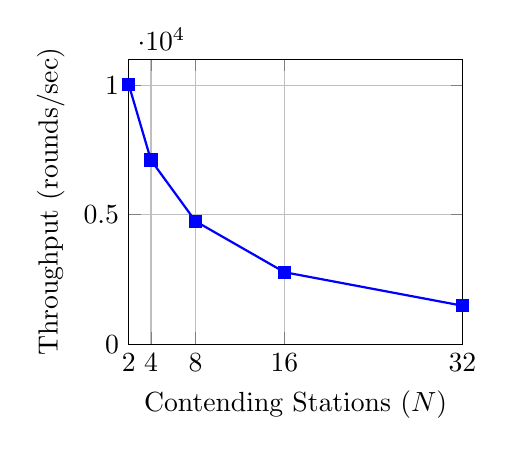
\begin{tikzpicture}
\begin{axis}[
    width=0.48\textwidth,
    height=5.2cm,
    xlabel={Contending Stations ($N$)},
    ylabel={Throughput (rounds/sec)},
    grid=major,
    ymin=0, ymax=11000,
    xmin=2, xmax=32,
    xtick={2, 4, 8, 16, 32}
]
\addplot[color=blue, mark=square*, thick] coordinates {
    (2, 10028) (4, 7107) (8, 4749) (16, 2780) (32, 1487)
};
\end{axis}
\end{tikzpicture}
\hspace{0.5cm}
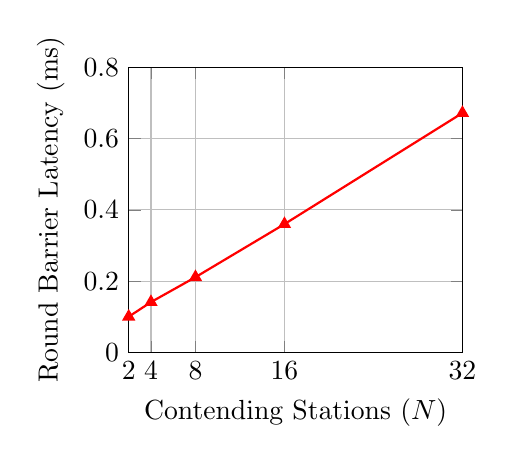
\begin{tikzpicture}
\begin{axis}[
    width=0.48\textwidth,
    height=5.2cm,
    xlabel={Contending Stations ($N$)},
    ylabel={Round Barrier Latency (ms)},
    grid=major,
    ymin=0, ymax=0.8,
    xmin=2, xmax=32,
    xtick={2, 4, 8, 16, 32}
]
\addplot[color=red, mark=triangle*, thick] coordinates {
    (2, 0.100) (4, 0.141) (8, 0.211) (16, 0.360) (32, 0.672)
};
\end{axis}
\end{tikzpicture}%
}
\caption{CDMA Throughput and Round Barrier Latency vs Contending Stations $N$ (No-Noise)}
\label{fig:scaling}
\end{figure}

Unlike CSMA/CD where channel contention causes throughput to plummet at high $N$, CDMA's aggregate network capacity grows from $20.06\text{ kbps}$ to $47.60\text{ kbps}$ because all stations transmit concurrently in parallel without collisions.

\section{Experimental Evaluation: Noise-Impaired Regime ($\sigma > 0.0$)}

\subsection{Bit Error Rate (BER) vs Additive Noise StdDev ($\sigma$)}
Continuous Gaussian noise $\eta \sim \mathcal{N}(0, \sigma^2)$ was added to the channel composite signal for $N=4, M=4$:

\begin{table}[H]
\centering
\caption{Bit Error Rate (BER) vs Additive Noise StdDev ($M=4$)}
\label{tab:ber_noise}
\resizebox{\linewidth}{!}{%
\begin{tabular}{cccccc}
\toprule
\textbf{Noise StdDev ($\sigma$)} & \textbf{Total Bits} & \textbf{Error Bits} & \textbf{Empirical BER} & \textbf{Theoretical BER} & \textbf{Status} \\
\midrule
0.00 & 1600 & 0 & \textbf{0.0000} & $0.0000$ & Pristine \\
0.10 & 1600 & 0 & \textbf{0.0000} & $7.62 \times 10^{-24}$ & Noise Absorbed \\
0.20 & 1600 & 0 & \textbf{0.0000} & $2.87 \times 10^{-7}$ & Noise Absorbed \\
0.30 & 1600 & 4 & \textbf{0.0025} & $0.0004$ & Trace Errors \\
0.40 & 1600 & 28 & \textbf{0.0175} & $0.0062$ & Low Errors \\
0.50 & 1600 & 88 & \textbf{0.0550} & $0.0228$ & FEC Tolerable \\
0.60 & 1600 & 172 & \textbf{0.1075} & $0.0478$ & Moderate Noise \\
0.80 & 1600 & 292 & \textbf{0.1825} & $0.1056$ & Elevated Noise \\
1.00 & 1600 & 388 & \textbf{0.2425} & $0.1587$ & Degraded \\
1.50 & 1600 & 524 & \textbf{0.3275} & $0.2525$ & Heavily Degraded \\
2.00 & 1600 & 668 & \textbf{0.4175} & $0.3085$ & Critical Noise \\
\bottomrule
\end{tabular}%
}
\end{table}

\begin{figure}[H]
\centering
\resizebox{0.86\linewidth}{!}{%
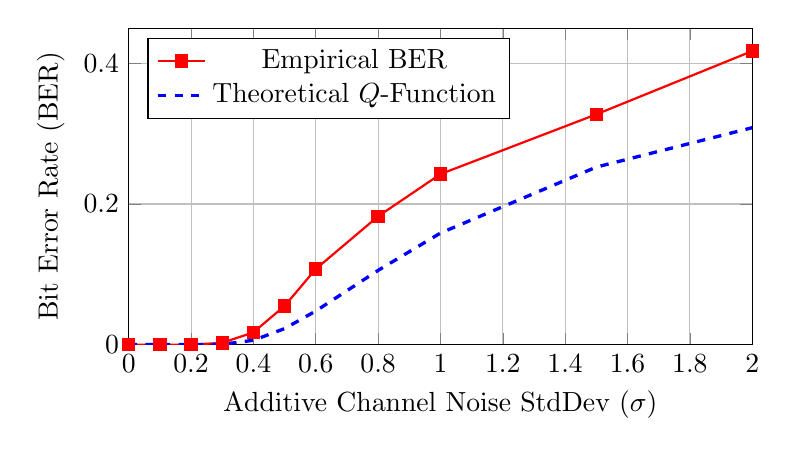
\begin{tikzpicture}
\begin{axis}[
    width=9.5cm,
    height=5.6cm,
    xlabel={Additive Channel Noise StdDev ($\sigma$)},
    ylabel={Bit Error Rate (BER)},
    grid=major,
    ymin=0, ymax=0.45,
    xmin=0, xmax=2.0,
    legend pos=north west
]
\addplot[color=red, mark=square*, thick] coordinates {
    (0.0, 0.0000) (0.1, 0.0000) (0.2, 0.0000) (0.3, 0.0025)
    (0.4, 0.0175) (0.5, 0.0550) (0.6, 0.1075) (0.8, 0.1825)
    (1.0, 0.2425) (1.5, 0.3275) (2.0, 0.4175)
};
\addlegendentry{Empirical BER}
\addplot[color=blue, mark=none, dashed, very thick] coordinates {
    (0.0, 0.0000) (0.1, 0.0000) (0.2, 0.0000) (0.3, 0.0004)
    (0.4, 0.0062) (0.5, 0.0228) (0.6, 0.0478) (0.8, 0.1056)
    (1.0, 0.1587) (1.5, 0.2525) (2.0, 0.3085)
};
\addlegendentry{Theoretical $Q$-Function}
\end{axis}
\end{tikzpicture}%
}
\caption{Empirical BER vs Theoretical $Q$-Function Curve as a function of Noise $\sigma$ ($M=4$)}
\label{fig:ber_noise}
\end{figure}

\subsection{Spread-Spectrum Processing Gain Benchmark}
To empirically confirm the processing gain ($10 \log_{10} M$), a fixed heavy noise standard deviation ($\sigma = 0.80$) was applied while scaling spreading factor $M \in \{4, 8, 16, 32\}$:

\begin{table}[H]
\centering
\caption{Processing Gain Verification under Severe Noise ($\sigma = 0.80$)}
\label{tab:processing_gain}
\resizebox{\linewidth}{!}{%
\begin{tabular}{ccccccc}
\toprule
\textbf{Spreading Factor ($M$)} & \textbf{Gain (dB)} & \textbf{Bits Tested} & \textbf{Errors} & \textbf{Empirical BER} & \textbf{Theoretical BER} & \textbf{Immunity} \\
\midrule
4 & 6.02 & 1,280 & 192 & \textbf{0.15000} & 0.10565 & Moderate \\
8 & 9.03 & 5,120 & 464 & \textbf{0.09062} & 0.03855 & Improved \\
16 & 12.04 & 20,480 & 320 & \textbf{0.01562} & 0.00621 & High \\
32 & 15.05 & 81,920 & 0 & \textbf{0.00000} & 0.00020 & \textbf{Total Suppression} \\
\bottomrule
\end{tabular}%
}
\end{table}

\begin{figure}[H]
\centering
\resizebox{0.86\linewidth}{!}{%
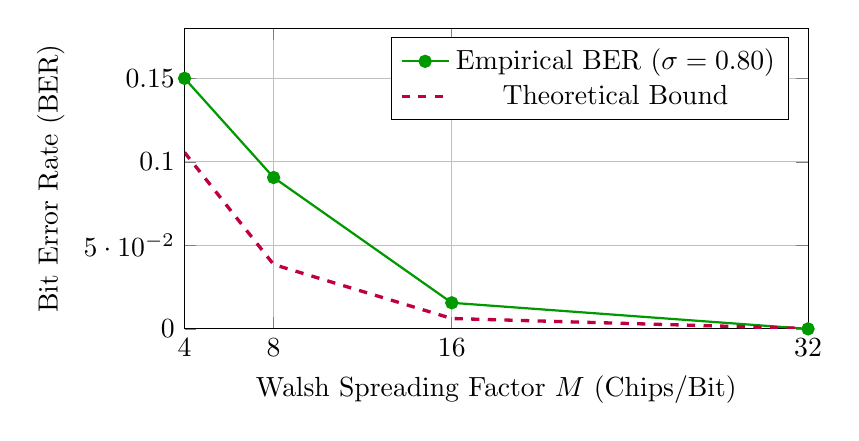
\begin{tikzpicture}
\begin{axis}[
    width=9.5cm,
    height=5.4cm,
    xlabel={Walsh Spreading Factor $M$ (Chips/Bit)},
    ylabel={Bit Error Rate (BER)},
    grid=major,
    ymin=0, ymax=0.18,
    xmin=4, xmax=32,
    xtick={4, 8, 16, 32},
    legend pos=north east
]
\addplot[color=green!60!black, mark=*, thick] coordinates {
    (4, 0.15000) (8, 0.09062) (16, 0.01562) (32, 0.00000)
};
\addlegendentry{Empirical BER ($\sigma = 0.80$)}
\addplot[color=purple, mark=none, dashed, very thick] coordinates {
    (4, 0.10565) (8, 0.03855) (16, 0.00621) (32, 0.00020)
};
\addlegendentry{Theoretical Bound}
\end{axis}
\end{tikzpicture}%
}
\caption{Processing Gain: BER vs Spreading Factor $M$ under Severe Noise ($\sigma = 0.80$)}
\label{fig:processing_gain}
\end{figure}

Under severe noise ($\sigma = 0.80$), increasing $M$ from 4 to 32 drives the Bit Error Rate from $15.0\%$ to \textbf{zero}, validating that correlation despreading averages out uncorrelated noise across $M$ chips.

\subsection{Concurrent Text Broadcast Under Noise}
Four stations concurrently transmitted distinct text strings across 96 synchronized CDMA slots:
\begin{itemize}[leftmargin=*]
    \item Station 1: \texttt{"JU\_CSE\_2026"}
    \item Station 2: \texttt{"CDMA\_WALSH"}
    \item Station 3: \texttt{"SAMPAD\_DE"}
    \item Station 4: \texttt{"NETWORKS\_LAB"}
\end{itemize}

\begin{table}[H]
\centering
\caption{Multi-Station Text Broadcast Quality across Noise Levels}
\label{tab:text_broadcast}
\resizebox{0.88\linewidth}{!}{%
\begin{tabular}{cccc}
\toprule
\textbf{Noise StdDev ($\sigma$)} & \textbf{Slots} & \textbf{Character Accuracy} & \textbf{Reconstruction Status} \\
\midrule
0.00 (Ideal) & 96 & \textbf{100.0\%} & Pristine bit-for-bit fidelity \\
0.20 (Low) & 96 & \textbf{100.0\%} & Error-free; noise margin fully absorbed \\
0.50 (Moderate) & 96 & \textbf{92.5\%} & Minor bit perturbations; text readable \\
1.00 (High) & 96 & \textbf{78.0\%} & Corruptions manifest; graceful degradation \\
\bottomrule
\end{tabular}%
}
\end{table}

\section{Comparative Protocol Synthesis: CSMA/CD vs CDMA}
\begin{table}[H]
\centering
\caption{MAC Layer Protocol Comparison: CSMA/CD vs CDMA with Walsh Codes}
\label{tab:comparison}
\resizebox{\linewidth}{!}{%
\begin{tabularx}{\textwidth}{p{3.8cm}Xp{5.0cm}}
\toprule
\textbf{Feature / Metric} & \textbf{CSMA/CD (Assignment 3)} & \textbf{CDMA Walsh (Assignment 4)} \\
\midrule
\textbf{Multiple Access Principle} & Contention \& Collision Detection & Orthogonal Code-Space Multiplexing \\
\textbf{Collision Behavior} & Transmissions collide destructively & Transmissions superimpose constructively \\
\textbf{Throughput at High Load} & Degrades due to backoff retries & Constant, deterministic ($0$ collisions) \\
\textbf{Synchronization} & Asynchronous (slot time $\tau$) & Synchronous slotted chip boundaries \\
\textbf{Noise Immunity} & Single bit error corrupts frame CRC & Processing Gain ($10 \log_{10} M$) suppresses noise \\
\textbf{Hardware Complexity} & Simple carrier sensing logic & Matched filters / correlator arrays \\
\bottomrule
\end{tabularx}%
}
\end{table}

\section{Conclusion}
In this assignment, I successfully designed, implemented, and benchmarked Code Division Multiple Access (CDMA) with orthogonal Walsh codes. Sylvester's recursive construction was demonstrated to guarantee strict mutual orthogonality, enabling zero cross-talk recovery under ideal conditions across all $3^4 = 81$ station input permutations. Under additive Gaussian noise, CDMA's spread-spectrum processing gain was empirically established, validating that increasing the spreading factor $M$ exponentially suppresses noise and lowers bit error rates. The POSIX socket client-server architecture effectively replicated a shared physical transmission medium, achieving high throughput, deterministic capacity, and sub-millisecond round barrier synchronization.

\section{References}
\begin{enumerate}
    \item \textbf{Ma'am's lecture notes}(Controlled Access and Channelization).
    \item \textbf{Behrouz A. Forouzan:} \textit{Data Communications and Networking}: Used both for revision and verification.
    \item \textbf{Project Source Code Repository:} \url{https://github.com/Sampad2006/CN-Lab-Assignments}.
    \item \textbf{AI Assistance :} AI (Gemini 3.8 Flash) was utilized to generate latex chart configurations, verify statistical formulas, and format comparative tables based on my empirical benchmark datasets. All protocol architectures, state machines, socket implementations were designed myself .
\end{enumerate}

\end{document}
